



\chapter{Estado de arte}





\section{Sistema de controlo de versões}

\subsection{Soluções livres}
CVS, Mercurial, Git e SVN


\subsection{Soluções comerciais}
SourceSafe, TFS, PVCS (Serena) e ClearCase


\subsection{Solução adoptada}





\section{Sistema de gestão de base de dados}


\subsection{PostgreSQL}


\subsection{SQL server}



\subsection{Solução adoptada}



\section{Framework de desenvolvimento web}


Manipulação local usando JS do DOM
Angular, React

Servidor serve conteudos criados em função dos pedidos do cliente 





\section{Frameworks/Tecnologias de desenvolvimento mobile}



\section{Android nativo}

\section{IOS nativo}

\section{Multi-plataforma}

\subsection{title}


http://websocialdev.com/lista-de-frameworks-para-desenvolvimento-mobile/




\section{API web}


\chapter{Sistema de controlo e monitorização}


\section{Design funcional}











\subsection{Requisitos funcionais}

\subsection{Requisitos não funcionais}







\section{Design técnico}



\subsection{Arquitetura do sistema}



\subsubsection{Camada de apresentação}


\subsubsection{Camada de negócio}



\subsubsection{Camada de dados}




\section{Diagrama de componentes}




\section{Sistema de interação}


\section{Descrição}


Modulos da daniela : Cc1110



\section{Arquitetura geral}

\begin{figure}[!htb]
	\centering
	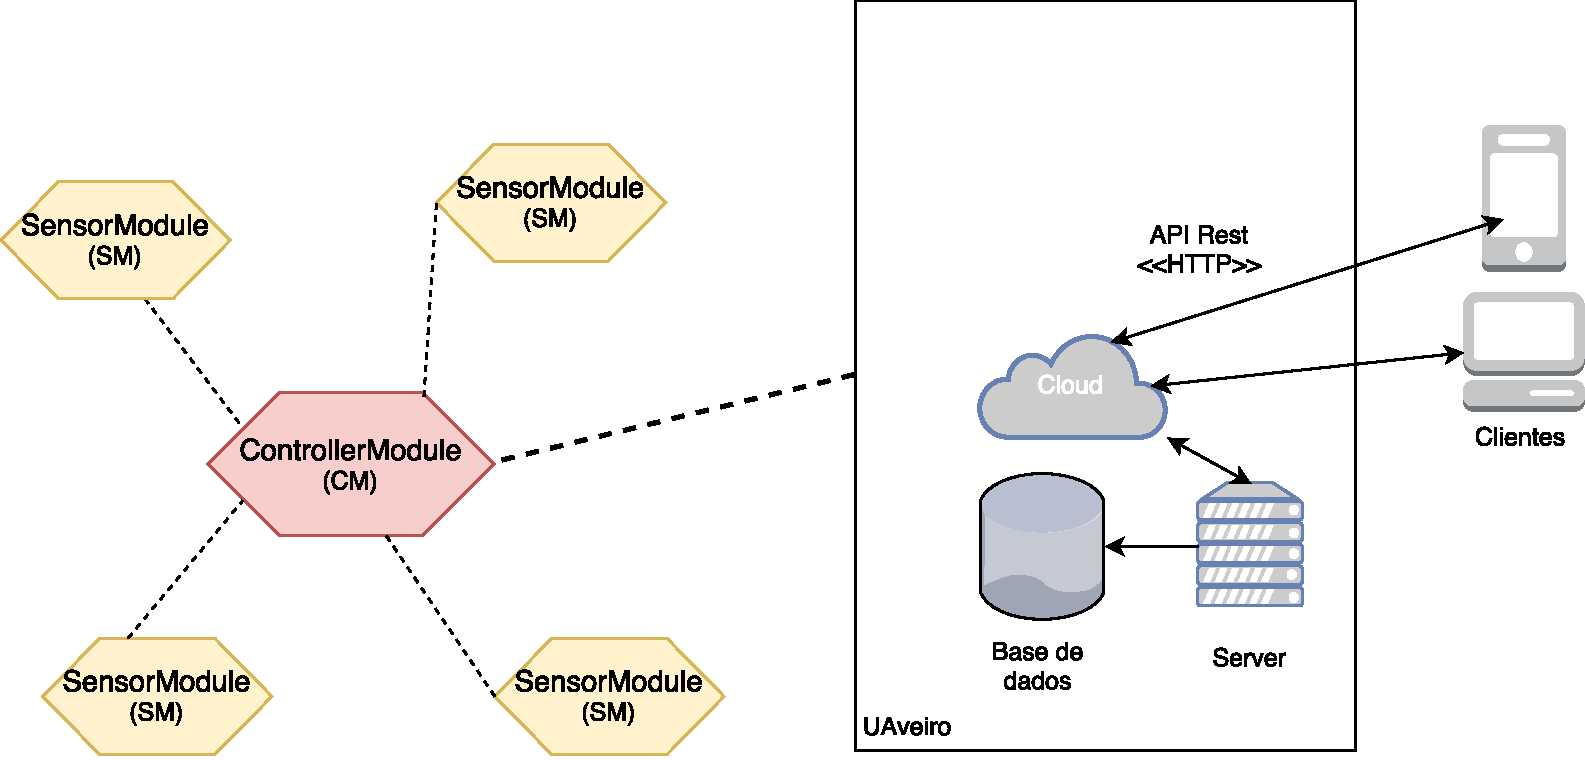
\includegraphics[scale=0.55]{esquemas/arquitetura_geral.pdf}
	\caption{Pirâmide do conhecimento: modelo DIKW}
	\label{dikw}
\end{figure}


\newpage


\section{Componentes}


\begin{figure}[!htb]
	\centering
	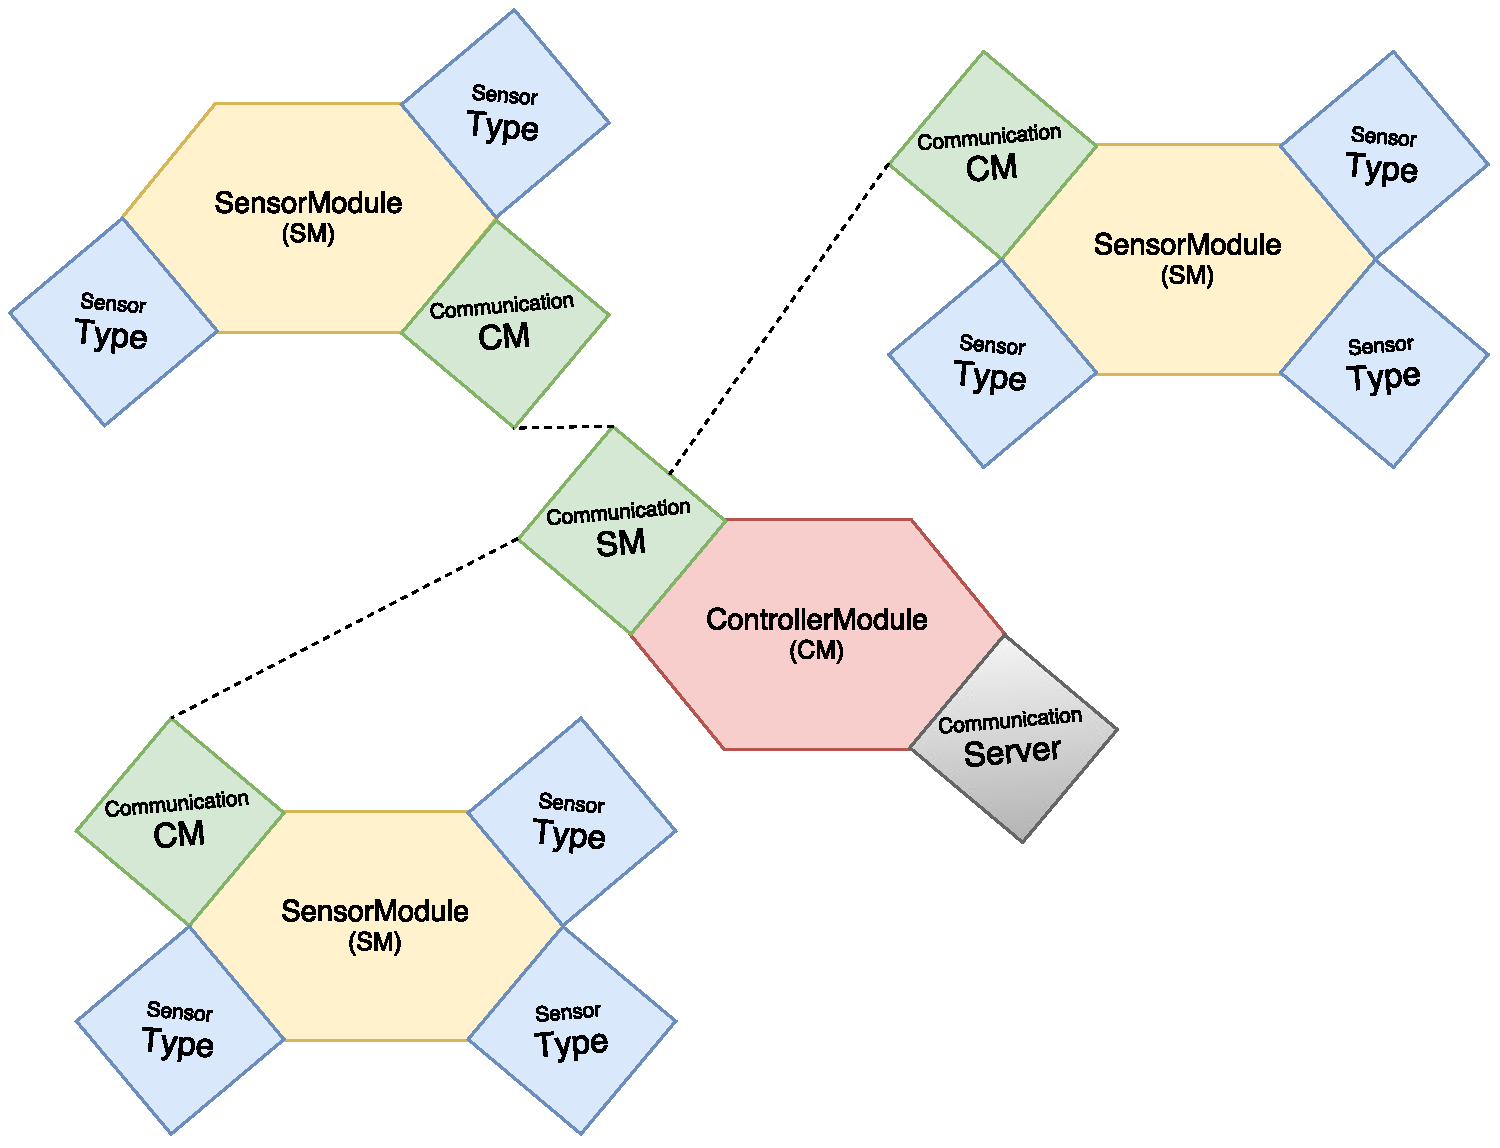
\includegraphics[scale=0.55]{esquemas/general-electronic-modules.pdf}
	\caption{Pirâmide do conhecimento: modelo DIKW}
	\label{dikw}
\end{figure}


\section{title}